\chapter{Estado del Arte}
 %\addcontentsline{toc}{chapter}{Estado del Arte}

En la actualidad las empresas en Colombia usan las computadoras y el Internet más que antes, se estima que de 8659 empresas el 99\% posee computador y está conectada a Internet \cite{Ardila2015}. En la Figura \ref{Ardila2015} se muestran los indicadores básicos de tenencia y uso de la información y la comunicación en las empresas. 
\begin{figure}[ht]
\centering
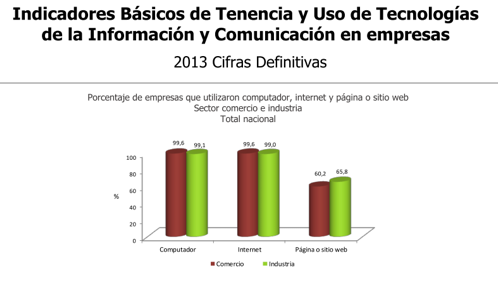
\includegraphics[width=10cm, height=8cm]{Ardila2015}
\caption{Indicadores básicos de tenencia y uso de la información y la comunicación en las empresas Colombianas en 2013.}
\label{Ardila2015}
\end{figure}
	
El Ministerio de Tecnologías de la información y las comunicaciones ha invertido hasta \$373993 millones de pesos colombianos hasta marzo del 2014 solo en el proyecto de conectividad de alta velocidad, el cual busca que el 100\% de los municipios del país tengan acceso a Internet de alta velocidad \cite{Comunicaciones2014}. 

Hace 50 años el análisis estadístico multivariado hubiera usado métodos lineales para descubrir el conocimiento almacenado en los datos históricos que se generan por las aplicaciones y el Internet, lamentablemente esta cantidad de datos hubiera sido un problema en esa época. Desde los años setenta los computadores se usaron en el análisis exploratorio de los datos y en las décadas posteriores fuimos testigos de un avance en el procesamiento y el almacenamiento de las computadoras, lo que permitió que grandes cantidades de datos fueran clasificados, almacenados y administrados de forma eficiente por los paquetes interactivos de software estadísticos, esto facilitó el análisis avanzado de los datos sin mucho esfuerzo, los procesos de extracción, transformación y carga fueron más comunes, los datos de máquina y la internet dieron inicio a nuevas disciplinas como la minería de datos y el aprendizaje estadístico. Actualmente, el análisis computacional de los datos está ganando popularidad. Las enormes cantidades de datos son cada vez más comunes y aunque las personas encargadas de analizarlos siguen teniendo en cuenta las técnicas supervisadas,  el descubrimiento de información no supervisado es la nueva tendencia. Como consecuencia, la estadística multivariada incluye nuevas técnicas desde las ciencias de la computación, muchas de ellas aún en su etapa de desarrollo. Los orígenes de estas técnicas son algoritmos derivados del modelado, la optimización y el razonamiento probabilístico, el desarrollo constante de las comunidades en el área han madurado y convertido la minería de datos, el aprendizaje estadístico y la inteligencia artificial en un excelente marco de trabajo \cite{Hastie2009}.

En este documento inicialmente se exploran varios ejemplos del uso de la minería de datos en las líneas de producto con el fín de evidenciar la pertinecia de este estudio, luego en los resultados se presenta el desarrollo del protocolo de la revisión sistematica de la literatura y se hace enfasis en nuestro ejemplo. En este apartado, Se partirá de un ambiente heterogéneo, donde existen diferentes compañías que desarrollan productos masivamente y pueden usar  muchas técnicas de análisis de datos en común \cite{Thum2014}, como funciones descriptivas, predictivas y técnicas  asociativas. 

\section{Algunos ejemplos sobre  compañías que quisieron adoptar las técnicas de minería de datos y la ingeniería de lineas de producto para incluirlo en el software que desarrolla sus productos} 

\begin{enumerate}
\item \textbf{\textit{Creación de un sistema de puntuación (Banco de Irán).}} Por lo general cuando se quiere aspirar a un crédito en una entidad financiera, los usuarios son puestos bajo un sistema de puntuación, estos son algoritmos dentro de los métodos clasificatorios, que preparan los datos del usuario o los alistan para un proceso posterior. Estos decrementos en la cantidad de datos a procesar, reducen el costo de cómputo que puedan generar las grandes cantidades de datos. Su aplicación es sencilla y su actualización también lo es. La información de los usuarios es ingresada a un modelo que propone el mejor producto crediticio según el comportamiento del usuario, su historial, sus productos o sus relaciones con otras entidades financieras. Mientras exista variabilidad se puede ver un sistema como una línea de productos y la minería de datos puede extraer las variabilidades de un sistema \cite{Koutanaei2015}.

\item \textbf{\textit{Planeando nuevas generaciones de productos (Apple).}} Para planear nuevas generaciones de productos, es decir planear la existencia de un determinado producto en el mercado, se deben tener en cuenta todas las características que lo conforman, el color, el precio y el tamaño.  El iPhone es un producto que quiere preservar su estado en el mercado, ser reconocido a lo largo del tiempo por ser novedoso y agrupar las mejores características; los usuarios generan los datos que ayudan a conocer sus necesidades y este conocimiento impulsa el desarrollo de nuevos productos como las tablets y de nuevos paradigmas como los Modelos variables de estados dinámicos.  Para implementarlos se necesita conocer el historial de las ventas y encontrar su tendencia, según la línea de producto se modela el sistema como un modelo de canibalización, este modelo consume los datos extraídos, busca las características que generan mayor beneficio económico y desecha las que no. Habiendo definido el modelo de canibalización es el turno de la iteración hacia adelante de Monte Carlo, con este algoritmo se originan las generaciones necesarias para que los productos sean competitivos en el mercado \cite{Lin2013}.

\item \textbf{\textit{Desarrollando productos con técnicas de minería de datos (cámara digital).}} Con los crecientes avances en la tecnología, los ciclos de vida de desarrollo de los productos deben hacerse cada vez más rápido, generando mayores ingresos, construyendo productos de mayor calidad, reduciendo el costo de producción y orientando los productos a las necesidades del cliente. Es en estas necesidades donde están las pistas para el mejoramiento del ciclo de vida del proceso de desarrollo de nuevos productos \cite{Davril2015b}. En el proceso de construcción de una cámara digital se pregunta ¿qué quiere o necesita un cliente de una cámara?¿Cuáles características son más importantes que otras? ¿Puede integrarse el diseño de los productos con lo que saben los clientes? ¿Cómo pueden estas reglas ayudar a mejorar el diseño de una cámara?  Antes de que un producto sea diseñado, muchas compañías tienen en cuenta los datos almacenados en bases de datos multidimensionales para responder las preguntas anteriores y validar sus hipótesis. Además, usan técnicas de la minería de datos que en el contexto de la clasificación, estimación, segmentación y descripción preparan los datos para ser minados, es decir para extraer conocimiento y por ejemplo en el caso de la cámara digital, planear la construcción de una línea de productos \cite{Bae2011}. 

\end{enumerate}

Teniendo en cuenta el desarrollo de los modelos de carateristicas, en la minería de datos pueden encontrarse características que están relacionadas de forma interesante y pueden ser modeladas mediante árboles de decisión \cite{Farid2014} y reglas de asociación \cite{Bhuyan2015}. Además, se sabe que estas características pueden estar asociadas a un beneficio económico \cite{Jiao2005}, y con esta asociación se puede usar un proceso de canibalización o de clasificación, desde el punto de vista de la información que está relacionada con las características específicas que logran el beneficio económico \cite{Lin2013}. En los ejemplos anteriores los datos que son sometidos a un proceso de evaluación, generan un patrón de decisión que elimina la redundancia en la información. Cuando se tienen las reglas de agrupamiento se inicia el proceso de construcción del modelo de características, el cual, acompañado de un marco de trabajo, finalmente genera las estrategias de diseño de los nuevos productos \cite{Chen2014a}.

Los ejemplos mencionados en el desarrollo de este estado del arte están orientados a la extracción de las características por medio del proceso CRISP, en el cual los datos históricos que son usados actualmente tienen muchos formatos y es preciso adaptar este proceso a la extracción del conocimiento de forma novedosa. La oportunidad de innovar depende del mejoramiento de la arquitectura CRISP para que incorpore un nuevo proceso de descubrimiento de las características mediante nuevos algoritmos de agrupamiento, debido a que normalmente no se conocen las clases o la cantidad de grupos de las mismas y que lo más popular es determinar este número mediante cross validation \cite{Fan2014} y shrinkage \cite{Simpson}. Por lo tanto, para plantear una estrategia que genere nuevos productos a partir de los datos históricos se presentan a continuación en el siguiente capitulo los siguientes objetivos de este proyecto de investigación.
